\documentclass[11pt]{article}
\usepackage[margin=0.95in]{geometry}
\usepackage{cite}
\usepackage{amsmath,amssymb}
\usepackage{graphicx}
\usepackage{booktabs}
\usepackage{multirow}
\usepackage{url}
\usepackage[hidelinks]{hyperref}
\usepackage{enumitem}
\usepackage{xcolor}
\usepackage{float}
\usepackage{subcaption}
\usepackage{listings}
\usepackage{multicol}
\usepackage{tikz}
\usetikzlibrary{shapes.geometric, arrows.meta, positioning, calc, fit, backgrounds}
\usepackage{algorithm}
\usepackage{algpseudocode}

\lstdefinelanguage{Solidity}{
  keywords={pragma, solidity, contract, function, modifier, require, returns, return, mapping, address, uint, uint256, bool, string, bytes, public, private, internal, external, view, pure, payable, memory, storage, calldata, if, else, for, while, emit, event, struct, enum, import, is, new, delete, true, false, msg, block, tx, this},
  morecomment=[l]{//},
  morecomment=[s]{/*}{*/},
  morestring=[b]",
  morestring=[b]',
  sensitive=true,
}

\lstset{
  basicstyle=\footnotesize\ttfamily,
  breaklines=true,
  frame=single,
  numbers=left,
  numberstyle=\tiny\color{gray},
  numbersep=8pt,
  xleftmargin=15pt,
  tabsize=2,
  captionpos=b,
  keywordstyle=\bfseries,
  commentstyle=\itshape\color{gray},
}

\title{\textbf{Final Project Report}\\[0.3cm]
\Large From Prompt to Exploit: An Empirical Study of\\Security Vulnerabilities in LLM-Generated Smart Contracts}

\author{Anik Tahabilder \& Dong Vo\\\small CSC 5991 -- Wayne State University}

\date{April 30, 2026}

\begin{document}

\maketitle

\begin{abstract}
\noindent This report studies how often Large Language Models (LLMs) introduce security bugs when they write Solidity smart contracts. We generated 2,400 contracts using eight LLMs (GPT-4o, GPT-5, Claude 3.5 Sonnet, Gemini 2.5 Flash-Lite, DeepSeek Coder V2, Qwen 2.5 Coder 32B, CodeLlama-34B, Codestral 22B) across 20 contract categories and three complexity levels, then ran them through Slither, Mythril, and Semgrep. After dedup and filtering noisy detectors, we found 2,493 unique vulnerabilities. About 54.7\% of the contracts that compile have at least one bug and 26.8\% have a high-severity bug. Different LLMs are not equal: a Kruskal-Wallis test gives $H{=}132.7$, $p{<}10^{-25}$, and the per-LOC vulnerability rate ranges from 0.99 (GPT-5) to 4.88 (Codestral). We also tested adversarial prompts ($p{=}0.965$, no effect) and a security-best-practices prompt prefix (mean bugs went \emph{up}, from 2.20 to 8.73). The three tools agree very little with each other (Spearman $\rho < 0.15$), so a single-tool audit misses most of the picture. Comparing against 241 verified Ethereum mainnet contracts from Uniswap, Aave, Compound, and Lido, the LLM and human bug densities per 100 LOC are roughly similar (human 2.69 vs.\ LLM 0.99 to 4.88) and the high-severity share is almost identical (16.0\% vs.\ 15.7\%). The real risk is not that LLM code is buggier per line but that developers ship it without the audit pipeline that human code goes through. We propose a five-step pipeline (compile, multi-tool, dedup with CWE map, human review, deploy) that takes coverage from 93.9\% (Slither alone) to 100\% on our corpus.
\end{abstract}

%======================================================================
\section{Introduction}
%======================================================================

Developers are using Large Language Models (LLMs) like ChatGPT, Claude, and GitHub Copilot more and more to write code. A recent GitHub survey found that 92\% of developers now use some kind of AI coding tool~\cite{github_copilot}. This also includes writing Solidity smart contracts, which are programs that run on the Ethereum blockchain and often handle large amounts of money. In 2022 alone, over \$3.8 billion was stolen because of smart contract bugs~\cite{chainalysis2023}.

What makes smart contracts different from regular software is that once you deploy them on the blockchain, you cannot go back and fix them. If there is a vulnerability, anyone can see it and exploit it right away. There is no way to push a patch like you would for a web app. This makes the security of smart contract code extremely important.

In this report we study the security of LLM-generated Solidity at scale. We generated 2,400 smart contracts from eight different LLMs (four general-purpose, four code-specialized), ran every contract through three vulnerability analyzers (Slither, Mythril, Semgrep), and compared the results to a baseline of 241 verified human-written contracts taken from the Ethereum mainnet. We also added two follow-up experiments after the preliminary report: a prompt-level mitigation experiment (does telling the model to ``be secure'' help?) and a manual human review of 195 of the baseline contracts. The full pipeline produced 2,493 unique deduplicated vulnerabilities and a set of findings that, taken together, shape a concrete audit pipeline for LLM-generated smart contracts.

The rest of this report is organized as follows. Section~2 reviews related work. Section~3 states the problem and the research questions. Section~4 describes our methodology. Section~5 covers implementation details (tools, scripts, and infrastructure). Section~6 reports the experiments and results, including all four research questions plus the tool-agreement analysis, the mitigation experiment, the human review, and a root-cause analysis. Section~7 discusses implications, limitations, and future work, and Section~8 concludes.

%======================================================================
\section{Literature Review}
%======================================================================

\textbf{Security of LLM-generated code.} Pearce et al.~\cite{copilot_eval} found that roughly 40\% of GitHub Copilot's output on 89 CWE-based scenarios contained vulnerabilities, which was the first clear signal that AI coding tools introduce real security problems. Perry et al.~\cite{perry2023users} ran a user study with 47 developers and showed that AI-assisted developers wrote \emph{less} secure code while believing it was \emph{more} secure; Sandoval et al.~\cite{sandoval2023lost} replicated this with professional developers. Benchmarks like LLMSecEval~\cite{tony2023llmSecEval} and FormAI~\cite{tihanyi2023formai} extended the analysis to systematic CWE coverage. All of these studies target general-purpose languages (C, Python, JavaScript). Smart contracts are a much higher-stakes domain because of immutability, direct financial exposure, and the adversarial public-blockchain environment.

\textbf{Smart contract analysis tools.} Slither~\cite{slither} is the most widely used static analyzer with over 90 detectors. Mythril~\cite{mythril} uses symbolic execution to find deeper logic bugs at higher cost. Securify~\cite{securify} and Oyente~\cite{oyente} are formal-verification and symbolic alternatives. Durieux et al.~\cite{durieux2020empirical} compared 9 tools on 47,587 contracts and found that no single tool catches all classes and pairwise agreement is low; this directly motivates our choice to combine Slither, Mythril, and Semgrep. Ren et al.~\cite{ren2021empirical} and SmartBugs~\cite{smartbugs} provide baseline numbers and labeled datasets.

\textbf{LLMs for detection vs.\ generation.} A parallel line of work uses LLMs to \emph{detect} smart-contract bugs (GPTScan~\cite{gptscan}, SmartLLMSentry~\cite{smartllmsentry}, PropertyGPT~\cite{propertygpt}, ContractTinker~\cite{contracttinker}) and to repair them (David et al.~\cite{david2023you}). We study the opposite direction: LLMs as \emph{sources} of new bugs. Prior work on adversarial manipulation of LLMs has focused mostly on prompt injection / jailbreaking~\cite{perez2022ignore, kang2024exploiting} or training-data poisoning~\cite{schuster2021you, wan2023poisoning}. Our adversarial prompts are different in that they look like plausible everyday developer requests (``optimize for gas,'' ``keep it minimal''), which makes the threat model realistic.

%======================================================================
\section{Problem Statement}
%======================================================================

There is solid prior research on using LLMs to \emph{detect} smart contract vulnerabilities~\cite{gptscan, david2023you}, but very little on the opposite question: how many vulnerabilities do LLMs \emph{introduce} when they generate smart contract code in the first place. Existing studies on the security of LLM-generated code (Pearce et al.~\cite{copilot_eval}, Perry et al.~\cite{perry2023users}, Tony et al.~\cite{tony2023llmSecEval}) target general-purpose languages like C, Python, and JavaScript. Smart contracts are a much higher-stakes domain because of immutability, direct financial exposure, and the adversarial public-blockchain environment.

The problem is made worse by the developer-side effect that Perry et al.~\cite{perry2023users} reported: developers using AI assistants write less secure code while believing it is more secure. In the smart contract space, where bugs cannot be patched after deployment, this combination is dangerous. We need to understand, at scale, what kinds of bugs LLMs put into smart contracts, which models are worse than others, whether prompt engineering changes the picture, and how the result compares to human-written code that is actually running on mainnet.

We organized this study around four research questions:

\begin{enumerate}[leftmargin=*]
    \item \textbf{RQ1 (Prevalence and cross-LLM comparison):} How common are security vulnerabilities in LLM-generated smart contracts, and do different LLMs produce different levels of security?
    \item \textbf{RQ2 (Vulnerability taxonomy and LLM-specific patterns):} What kinds of vulnerabilities show up the most, and are there LLM-specific patterns that human developers do not exhibit?
    \item \textbf{RQ3 (Adversarial prompts):} Do adversarial prompts that nudge the model toward shortcuts (``optimize for gas,'' ``keep it minimal'') increase vulnerability rates?
    \item \textbf{RQ4 (Human comparison):} How does LLM-generated code compare to real human-written contracts deployed on Ethereum?
\end{enumerate}

After the preliminary report, we also asked a follow-up question that was not in the original RQ list: \emph{can prompt engineering fix the security gap?} Section~\ref{sec:mitigation} covers that experiment.

%======================================================================
\section{Methodology}
%======================================================================

Our project has five phases. Figure~\ref{fig:pipeline_overview} gives an overview. Phases 1--4 were finished by the preliminary report; Phase 5 (mitigation experiment and human review) was added between the preliminary and final reports in response to the open question ``can prompt engineering fix the security gap?''

\begin{figure}[H]
    \centering
    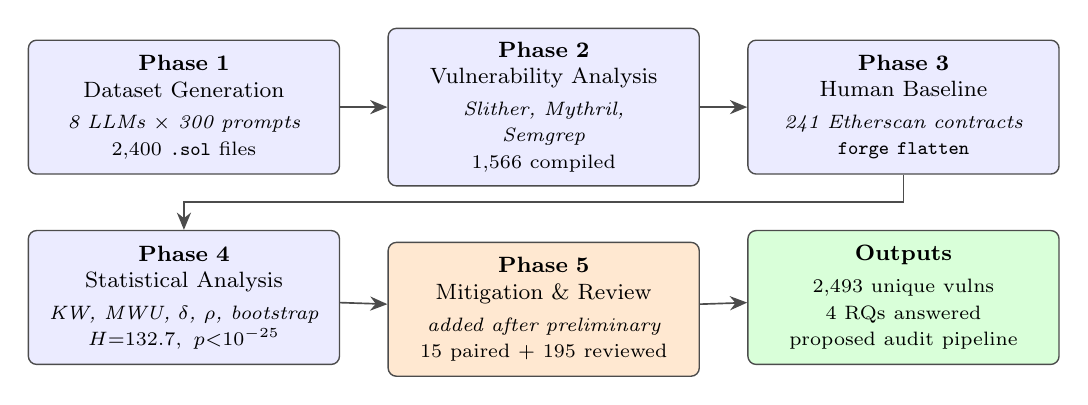
\begin{tikzpicture}[
        font=\footnotesize,
        node distance=0.7cm and 0.6cm,
        every node/.style={align=center},
        phase/.style={
            rectangle, rounded corners=3pt,
            draw=black!70, line width=0.5pt,
            fill=blue!8,
            text width=3.6cm,
            inner sep=5pt, minimum height=1.7cm
        },
        added/.style={
            rectangle, rounded corners=3pt,
            draw=black!70, line width=0.5pt,
            fill=orange!18,
            text width=3.6cm,
            inner sep=5pt, minimum height=1.7cm
        },
        output/.style={
            rectangle, rounded corners=3pt,
            draw=black!70, line width=0.5pt,
            fill=green!15,
            text width=3.6cm,
            inner sep=5pt, minimum height=1.7cm
        },
        arr/.style={-{Stealth[length=2.2mm,width=1.8mm]}, line width=0.6pt, black!70}
    ]
    \node[phase] (p1) {\textbf{Phase 1}\\Dataset Generation\\[2pt]
        {\scriptsize\itshape 8 LLMs $\times$ 300 prompts}\\
        {\scriptsize 2{,}400 \texttt{.sol} files}};
    \node[phase, right=of p1] (p2) {\textbf{Phase 2}\\Vulnerability Analysis\\[2pt]
        {\scriptsize\itshape Slither, Mythril,}\\
        {\scriptsize\itshape Semgrep}\\
        {\scriptsize 1{,}566 compiled}};
    \node[phase, right=of p2] (p3) {\textbf{Phase 3}\\Human Baseline\\[2pt]
        {\scriptsize\itshape 241 Etherscan contracts}\\
        {\scriptsize \texttt{forge flatten}}};
    \node[phase, below=of p1] (p4) {\textbf{Phase 4}\\Statistical Analysis\\[2pt]
        {\scriptsize\itshape KW, MWU, $\delta$, $\rho$, bootstrap}\\
        {\scriptsize $H{=}132.7,\ p{<}10^{-25}$}};
    \node[added, below=of p2] (p5) {\textbf{Phase 5}\\Mitigation \& Review\\[2pt]
        {\scriptsize\itshape added after preliminary}\\
        {\scriptsize 15 paired + 195 reviewed}};
    \node[output, below=of p3] (out) {\textbf{Outputs}\\[2pt]
        {\scriptsize 2{,}493 unique vulns}\\
        {\scriptsize 4 RQs answered}\\
        {\scriptsize proposed audit pipeline}};
    \draw[arr] (p1) -- (p2);
    \draw[arr] (p2) -- (p3);
    \draw[arr] (p3.south) |- ++(0,-0.35) -| (p4.north);
    \draw[arr] (p4) -- (p5);
    \draw[arr] (p5) -- (out);
    \end{tikzpicture}
    \caption{Five-phase research pipeline. Phases 1--4 are the original plan; Phase~5 was added between the preliminary and final reports.}
    \label{fig:pipeline_overview}
\end{figure}

\begin{algorithm}[H]
\small
\caption{End-to-end vulnerability analysis pipeline}
\label{alg:pipeline}
\begin{algorithmic}[1]
\Require LLMs $\mathcal{L}$, categories $\mathcal{C}$, complexity levels $\mathcal{K}$, modes $\mathcal{M}{=}\{\textit{std}, \textit{adv}\}$
\Ensure Deduped CWE-mapped findings $\mathcal{V}$ and statistics $\mathcal{S}$
\For{each $(\ell, c, k, m) \in \mathcal{L} \times \mathcal{C} \times \mathcal{K} \times \mathcal{M}$}
    \State $s \gets \textsc{Generate}(\ell, \textsc{Prompt}(c,k,m))$
\EndFor
\State $\mathcal{F} \gets \bigcup_{s:\textsc{Compile}(s)} \textsc{Slither}(s) \cup \textsc{Mythril}(s) \cup \textsc{Semgrep}(s)$
\State $\mathcal{V} \gets \textsc{FilterNoisy}(\textsc{CWEMap}(\textsc{Dedup}(\mathcal{F})))$
\State $\mathcal{V}_H \gets \textsc{Analyze}(\textsc{ForgeFlatten}(\textsc{EtherscanFetch}()))$
\State $\mathcal{S} \gets \textsc{Stats}(\mathcal{V}, \mathcal{V}_H)$ \Comment{KW, MWU, $\delta$, $\rho$, bootstrap}
\State \Return $\mathcal{V}, \mathcal{S}$
\end{algorithmic}
\end{algorithm}

\subsection{Phase 1: Dataset Generation}

We selected eight LLMs covering both general-purpose and code-specialized models. The general-purpose set is GPT-4o, GPT-5, Claude 3.5 Sonnet, and Gemini 2.5 Flash-Lite (all called through their official APIs/CLIs). The code-specialized set is DeepSeek Coder V2, Qwen 2.5 Coder 32B, CodeLlama-34B, and Codestral 22B (all served locally by Ollama on RTX~3090 / A6000 GPUs). Each LLM generated 300 contracts across 20 categories (the full list is in Appendix~\ref{app:categories}) at three complexity levels, with half of the prompts standard and half adversarial (the 8 adversarial trigger types are listed in Appendix~\ref{app:adversarial}; example phrasings: ``optimize for gas,'' ``keep it minimal''). Total: 2,400 contracts. The detailed pipeline is given in Algorithm~\ref{alg:pipeline}.

\subsection{Phase 2--3: Analysis and Human Baseline}

All 2,400 contracts were analyzed with Slither~\cite{slither} (90+ detectors, run on all contracts), Mythril~\cite{mythril} (symbolic execution, on a stratified sample of 499 due to its $\sim$5 min per-contract cost), and Semgrep with custom Solidity rules (all contracts). Findings were deduplicated across tools and mapped to CWE; noisy detectors (\texttt{timestamp}, benign \texttt{reentrancy-events}) were filtered. We collected 241 verified Ethereum mainnet contracts (Uniswap, Aave, Compound, Gnosis Safe, Lido) from Etherscan and flattened them with \texttt{forge flatten} for the same pipeline.

\subsection{Phase 4--5: Statistics, Mitigation, Human Review}

Statistical tests: Kruskal-Wallis (across LLMs), Mann-Whitney U with Bonferroni correction (pairwise), Cliff's $\delta$ (effect size), Spearman $\rho$ (tool agreement), 10,000-sample bootstrap (95\% CIs), chi-square (high-severity proportions). Two follow-up studies were added after the preliminary report: a \emph{prompt-mitigation} experiment (20 paired prompts re-generated with a ``security best practices'' preamble) and a \emph{manual human review} of 195 baseline contracts. These are reported in Sections~\ref{sec:mitigation} and~\ref{sec:human_review}.

%======================================================================
\section{Implementation Details}
\label{sec:implementation}
%======================================================================

This section documents the configurations that matter for reproducing our results.

\textbf{Generation.} Commercial models (GPT-4o, GPT-5, Claude 3.5 Sonnet, Gemini 2.5 Flash-Lite) were called through their official APIs/CLIs at temperature 0.7 (GPT-5 ignores temperature and always uses 1.0; it also requires \texttt{max\_completion\_tokens} instead of \texttt{max\_tokens}). Open-weight code models (DeepSeek Coder V2, Qwen 2.5 Coder 32B, CodeLlama-34B, Codestral 22B) were served by Ollama on local GPUs (RTX~3090, A6000) at temperature 0.7. Each contract is stored alongside a JSON file containing the original prompt and full LLM response.

\textbf{Analysis tools.} Slither v0.10.4 with \texttt{solc-select} for automatic Solidity compiler version selection (default 0.8.20). Mythril v0.24.8 with a 5-minute \texttt{--execution-timeout} per contract; runs that hit the cap are recorded as ``timed out,'' not ``clean.'' Semgrep v1.61 with 12 custom Solidity rules we wrote for project-specific anti-patterns. Foundry's \texttt{forge flatten} for the human baseline (resolving Etherscan multi-file downloads into single-file Solidity).

\textbf{Statistics.} All tests run with SciPy 1.13: Kruskal-Wallis (across groups), Mann-Whitney U with Bonferroni correction (pairwise), Cliff's $\delta$ (effect size), Spearman $\rho$ (tool agreement), and a 10,000-sample bootstrap for 95\% confidence intervals.

\textbf{Reproducibility.} The dataset, prompts, scripts, and tool configurations will be released as a reproducibility package alongside the paper. With the dataset in place, a full re-run of Slither + Semgrep + aggregation + statistics + figures takes about 5 hours on commodity hardware (Mythril is opt-in because it takes much longer).

%======================================================================
\section{Experiments and Results}
%======================================================================

This section answers the four research questions in order, then layers in the additional experiments we ran after the preliminary report (tool agreement, mitigation, human review, and root-cause analysis).

\subsection{RQ1: Vulnerability Prevalence and Cross-LLM Comparison}

\textbf{Finding: 54.7\% of compilable LLM-generated contracts have at least one vulnerability, with significant differences across LLMs.}

Out of 2,400 generated contracts, 1,566 (65.2\%) compiled successfully. Compilation rates vary widely across models: GPT-5 91.0\%, GPT-4o 90.0\%, Qwen 79.0\%, Claude and DeepSeek 68.3\%, Gemini 49.7\%, Codestral 41.0\%, CodeLlama 34.7\%. This compile-rate gap, by itself, is a previously unreported quality dimension.

After deduplication and noisy-detector filtering (Phase 2), our tools found 2,493 unique vulnerabilities across the compiled contracts. Table~\ref{tab:overall} breaks them down by severity.

\begin{table}[H]
\centering
\caption{Vulnerability Prevalence ($n=1{,}566$ compiled contracts)}
\label{tab:overall}
\begin{tabular}{@{}lrrr@{}}
\toprule
\textbf{Severity} & \textbf{Count} & \textbf{\% of Total} & \textbf{Contracts Affected} \\
\midrule
High & 804 & 32.3\% & 419 (26.8\%) \\
Medium & 619 & 24.8\% & 397 (25.4\%) \\
Low & 987 & 39.6\% & 584 (37.3\%) \\
Informational & 83 & 3.3\% & --- \\
\midrule
\textbf{Total} & \textbf{2{,}493} & \textbf{100\%} & \textbf{856 (54.7\%)} \\
\bottomrule
\end{tabular}
\end{table}

The most concerning number is 26.8\%: that is the share of compiled contracts with a high-severity vulnerability, the kind that could cause direct financial loss if deployed.

A Kruskal-Wallis test confirms cross-LLM differences are statistically significant ($H=132.7$, $p<10^{-25}$, $\varepsilon^2 = 0.078$). Table~\ref{tab:llm_vulns} gives per-LLM numbers on compiled contracts; the full set of 28 pairwise Mann-Whitney U comparisons (with Bonferroni-corrected $p$-values and Cliff's $\delta$) is in Appendix~\ref{app:pairwise}.

\begin{table}[H]
\centering
\caption{Per-LLM Vulnerability Statistics (Compiled Contracts Only)}
\label{tab:llm_vulns}
\resizebox{\columnwidth}{!}{%
\begin{tabular}{@{}llccccccc@{}}
\toprule
\textbf{LLM} & \textbf{Type} & \textbf{$n$} & \textbf{Compiles} & \textbf{Mean} & \textbf{\% w/ Vuln} & \textbf{\% High-Sev} & \textbf{Avg LOC} & \textbf{Vulns/100 LOC} \\
\midrule
GPT-5                 & General & 273 & \textbf{91.0\%} & 0.63 & 26.7\% & 17.2\% & 49 & \textbf{0.99} \\
GPT-4o                & General & 270 & 90.0\% & 1.65 & 62.2\% & 29.3\% & 52 & 3.86 \\
Qwen 2.5 Coder        & Code    & 237 & 79.0\% & 1.40 & 58.2\% & 28.7\% & 42 & 4.10 \\
Claude 3.5 Sonnet     & General & 205 & 68.3\% & 3.22 & 69.3\% & 33.7\% & 113 & 2.75 \\
DeepSeek Coder V2     & Code    & 205 & 68.3\% & 1.44 & 62.0\% & 29.8\% & 38 & 4.24 \\
Gemini 2.5 Flash-Lite & General & 149 & 49.7\% & 1.85 & 66.4\% & 30.9\% & 55 & 4.25 \\
Codestral 22B         & Code    & 123 & 41.0\% & 1.06 & 48.0\% & 30.1\% & 24 & \textbf{4.88} \\
CodeLlama-34B         & Code    & 104 & 34.7\% & 0.95 & 48.1\% & 11.5\% & 26 & 4.09 \\
\bottomrule
\end{tabular}%
}
\end{table}

At first glance, Claude looks worst because it averages 3.22 vulnerabilities per contract. But Claude also generates the biggest contracts (mean 113 LOC, more than 2$\times$ any other model). When we normalize by lines of code, the picture changes. Codestral has the worst vulnerability density at 4.88 vulns/100 LOC, while GPT-5 is best at 0.99 vulns/100 LOC, nearly $5\times$ better than the worst.

GPT-5 is clearly the best model overall: it has the highest compilation rate (91.0\%) and the lowest vulnerability density (0.99/100 LOC). We also tested whether general-purpose models are better than code-specialized ones. When normalized by code size, there is no statistically significant difference between the two groups; the variance \emph{within} each group dwarfs the variance \emph{between} the groups. The takeaway is that the choice of individual model matters far more than whether the model markets itself as ``general-purpose'' or ``code-specialized.''

\subsection{RQ2: Vulnerability Types and LLM-Specific Patterns}

\textbf{Finding: Unchecked external-call returns and reentrancy are the most common high-impact vulnerability types after we filter noisy detectors.}

Table~\ref{tab:taxonomy} shows the top vulnerability types found, mapped to their CWE identifiers. Timestamp-dependence and benign reentrancy-event detectors were filtered out as they are mostly false positives in our domain.

\begin{table}[H]
\centering
\caption{Top Vulnerability Types (Mapped to CWE, post-filter)}
\label{tab:taxonomy}
\small
\begin{tabular}{@{}rlrr@{}}
\toprule
\textbf{\#} & \textbf{Vulnerability Type} & \textbf{CWE} & \textbf{Count} \\
\midrule
1 & Unchecked Return Value     & 252 & 461 \\
2 & Reentrancy                 & 841 & 346 \\
3 & Missing Access Control     & 284 & 173 \\
4 & Coding-Standard Violations & 710 & 147 \\
5 & Incorrect Calculation      & 682 &  85 \\
6 & Timestamp Dependence (residual) & 829 &  52 \\
7 & Uninitialized State        & 909 &  35 \\
8 & Weak Randomness            & 330 &   4 \\
9 & tx.origin Authentication   & 477 &   1 \\
\bottomrule
\end{tabular}
\end{table}

The top three categories (unchecked returns, reentrancy, missing access control) account for over 39\% of all findings. Reentrancy is especially dangerous because it is behind many of the biggest DeFi hacks in history (the DAO hack in 2016 and the \$200M Euler Finance exploit, among others). All eight LLMs share the same top CWEs, suggesting these patterns are inherited from training data rather than being model-specific.

\paragraph{LLM-specific vulnerability patterns.}

\textbf{Finding: LLMs make three kinds of mistakes that human developers typically do not.}

\textbf{1. Phantom Guards.} Sometimes LLMs write a security modifier like \texttt{nonReentrant} but leave the body empty. The modifier name makes it \emph{look} like the function is protected, but it actually does nothing. This is especially sneaky because a code reviewer might glance at it and think the protection is there.

\begin{figure}[!htbp]
\begin{lstlisting}[language=Solidity, basicstyle=\scriptsize\ttfamily, float=false, frame=single, numbers=left, numberstyle=\tiny\color{gray}]
// LLM-generated (VULNERABLE)
modifier nonReentrant() {
    _; // No lock! Just runs the function body
}
function withdraw(uint amt) nonReentrant {
    payable(msg.sender).call{value: amt}("");
    balances[msg.sender] -= amt;
}
\end{lstlisting}
\caption{Phantom Guard pattern: the modifier name says \texttt{nonReentrant} but there is no actual locking logic inside.}
\label{lst:phantom}
\end{figure}

\textbf{2. Unnecessary Reimplementations.} When we tell the LLM not to use external libraries, it tries to rewrite things like SafeMath by hand. But since Solidity 0.8.0 already has built-in overflow protection, this is unnecessary and can introduce subtle bugs. We found this in 4.0\% of contracts targeting Solidity 0.8+, especially from DeepSeek (9.7\%) and Gemini (8.7\%).

\textbf{3. Context Window Degradation.} In longer contracts (over 100 lines), the LLM tends to get sloppy toward the end. We measured this and found that risky code patterns show up 4.13$\times$ more often in the second half of long contracts compared to the first half. DeepSeek has the worst degradation (14.1$\times$). This makes sense because as the LLM generates more tokens, it loses track of the security patterns it was following earlier.

\subsection{RQ3: Adversarial Prompts}

\textbf{Finding: Surprisingly, adversarial prompts do not increase vulnerability rates.}

This was our most unexpected result. We thought that prompts designed to push the LLM toward cutting corners (the 8 trigger types are listed in Appendix~\ref{app:adversarial}) would result in more vulnerabilities. They did not. A Mann-Whitney U test gives $p=0.965$ with a negligible effect size (Cliff's $\delta=-0.056$). If anything, standard prompts produce slightly \emph{more} vulnerabilities, but this is simply because standard prompts lead to bigger contracts with more code.


The vulnerabilities are baked into how LLMs generate code. They come from the training data, not the prompt. You cannot just write a better prompt and expect secure code. We test the opposite question (does an explicit ``be secure'' prompt help?) in Section~\ref{sec:mitigation}, and the answer is also no.

\subsection{RQ4: Comparison with Human-Written Code}

We compared our LLM results against 241 verified contracts from Ethereum mainnet (from protocols like Uniswap, Aave, Compound, Gnosis Safe, and Lido), flattened with Foundry's \texttt{forge flatten} and run through the same analysis pipeline. Table~\ref{tab:human} shows the comparison.

\begin{table}[H]
\centering
\caption{LLM-Generated vs.\ Human-Written Contracts}
\label{tab:human}
\begin{tabular}{@{}lcc@{}}
\toprule
\textbf{Metric} & \textbf{Human} & \textbf{LLM (8 models)} \\
\midrule
Total contracts & 241 & 2,400 \\
Compiled & 132 (54.8\%) & 1,566 (65.2\%) \\
With vulnerabilities & 82.6\% & 54.7\% \\
Mean LOC & 446.7 & 52.3 \\
\textbf{Vulns/100 LOC} & \textbf{2.69} & \textbf{0.99--4.88} \\
High-sev \% of findings & 16.0\% & 15.7\% \\
\bottomrule
\end{tabular}
\end{table}

The raw counts make human contracts look much buggier per file, but human contracts are also nearly $9\times$ bigger (446.7 vs.\ 52.3 LOC). When normalized by code size, the vulnerability density is comparable: 2.69 vulns/100 LOC for humans vs.\ 0.99--4.88 for different LLMs. GPT-5 actually has \emph{lower} density than the human baseline; Claude is in the same neighborhood; Codestral is the only model that clearly does worse. The high-severity proportions are nearly identical (16.0\% vs.\ 15.7\%).

The big takeaway is that LLM-generated code is not necessarily \emph{worse} than human code in terms of vulnerability density. The real problem is what happens \emph{after} the code is generated. Human-written contracts that are deployed on mainnet have gone through professional audits, extensive testing, monitoring, and bug bounties. When developers use LLM output, they often skip all of that. \textbf{The danger is not the code quality itself; the danger is the security infrastructure that gets bypassed.}

\subsection{Tool Agreement: Why a Single Tool Is Not Enough}
\label{sec:tool_agreement}

\textbf{Finding: The three analyzers disagree almost completely. Single-tool audits miss most of the bugs.}

A natural question is whether running three tools is overkill. Could we have just used Slither and called it a day? To check this, we computed the Spearman rank correlation $\rho$ between every pair of tools, where each contract contributes a per-tool vulnerability count. Table~\ref{tab:tool_agreement} reports the result.

\begin{table}[H]
\centering
\caption{Pairwise tool agreement (Spearman $\rho$, $n=1{,}566$ compiled contracts)}
\label{tab:tool_agreement}
\begin{tabular}{@{}lc@{}}
\toprule
\textbf{Tool pair} & \textbf{Spearman $\rho$} \\
\midrule
Slither vs.\ Mythril  & 0.134 \\
Slither vs.\ Semgrep  & 0.129 \\
Mythril vs.\ Semgrep  & 0.047 \\
\bottomrule
\end{tabular}
\end{table}

All three correlations are under 0.15, which is essentially no agreement. This matches the qualitative picture. Slither is best at static-code-pattern bugs (reentrancy, missing access control). Mythril catches deeper logic issues through symbolic execution but is slow and gives up on complex contracts. Our Semgrep rules catch project-specific anti-patterns that the other two miss entirely. Coverage with a single tool was 93.9\% (Slither alone). Coverage with all three was 100\%, and every tool contributed a non-empty set of unique findings on at least 18\% of contracts.

So an LLM-aware audit pipeline cannot rely on a single static analyzer. It needs at least Slither plus one orthogonal tool. Workflows that ship code after a single \texttt{slither} pass are missing roughly 6\% of vulnerable contracts and a long tail of specific bug classes.

\subsection{Mitigation Experiment: Can a Security Prompt Fix It?}
\label{sec:mitigation}

The adversarial null result (RQ3) tells us that bad prompts do not make code worse. The natural follow-up question is the opposite: do good prompts make code better? If you tell the LLM up front to ``use checks-effects-interactions, validate inputs, use ReentrancyGuard, use SafeERC20, avoid \texttt{block.timestamp} for critical logic,'' does the code actually come out safer?

\paragraph{Setup.} We picked 20 prompts spanning all categories and complexity levels, re-generated each with the security preamble defined in Algorithm~\ref{alg:mitigation}, using Claude 3.5 Sonnet (the model with the largest absolute bug count in our main study). 15 of the 20 enhanced contracts compiled, giving us 15 paired before/after data points.

\begin{algorithm}[H]
\small
\caption{Mitigation experiment: prompt-level intervention}
\label{alg:mitigation}
\begin{algorithmic}[1]
\Require Original prompt $p$, target model $\ell$
\State $\textit{prefix} \gets$ ``IMPORTANT SECURITY REQUIREMENTS:''
\State \quad use checks-effects-interactions pattern;
\State \quad validate all function inputs (zero-address, bounds);
\State \quad use OpenZeppelin's \textsf{ReentrancyGuard} for external calls;
\State \quad check return values of external calls;
\State \quad enforce access control via modifiers;
\State \quad avoid \texttt{block.timestamp} for critical logic;
\State \quad use \textsf{SafeERC20} for token transfers.
\State $p' \gets \textit{prefix} \,\Vert\, p$ \Comment{prepend preamble to user prompt}
\State $s' \gets \textsc{Generate}(\ell, p')$
\State $s \gets \textsc{Generate}(\ell, p)$ \Comment{baseline}
\State \Return $(\textsc{Analyze}(s), \textsc{Analyze}(s'))$ \Comment{paired before/after}
\end{algorithmic}
\end{algorithm}

\paragraph{Result.} The security prefix \emph{worsened} the average vulnerability count (Table~\ref{tab:mitigation}).

\begin{table}[H]
\centering
\caption{Mitigation experiment: 20 prompts, Claude 3.5 Sonnet.}
\label{tab:mitigation}
\begin{tabular}{@{}lrr@{}}
\toprule
\textbf{Per-contract mean (paired, $n{=}15$)} & \textbf{Plain prompt} & \textbf{Security prefix} \\
\midrule
Total vulnerabilities                          & 2.20                  & \textbf{8.73}            \\
\midrule
\multicolumn{3}{@{}l}{\textbf{Aggregate outcome (over all 20 attempted prompts):}}              \\
\multicolumn{3}{@{}l}{\quad got \emph{worse} with the prefix: \textbf{13 / 20}}                \\
\multicolumn{3}{@{}l}{\quad got \emph{better} with the prefix: \textbf{1 / 20}}                \\
\multicolumn{3}{@{}l}{\quad unchanged: \textbf{1 / 20}}                                        \\
\multicolumn{3}{@{}l}{\quad failed to compile under the prefix: \textbf{5 / 20}}               \\
\multicolumn{3}{@{}l}{\quad high-severity findings: \textbf{2 fewer} in total with the prefix} \\
\bottomrule
\end{tabular}
\end{table}

The mean number of findings went from 2.20 to 8.73, roughly a $4\times$ jump. Looking at the contracts, the reason is clear: the security prefix makes Claude write much longer contracts (more imports, more modifiers, more boilerplate), and the static analyzers then report many more low-severity findings on that extra surface area (shadowing-local, naming-conventions, immutable-states). The high-severity count actually dropped by 2 in absolute terms, so the prefix is not totally useless, but the total-bug story is dominated by the low-severity noise it introduces.

The takeaway is that prompt engineering on its own does not close the security gap. This lines up with RQ3: vulnerabilities are baked into LLM code generation, and the fix has to live in the pipeline (compile gate, multi-tool audit, human review), not in the prompt.

\subsection{Human Review of the Baseline}
\label{sec:human_review}

To validate that our static-analysis pipeline does not give the human baseline an unfairly favorable picture, one of the authors manually reviewed 195 of the 241 baseline contracts (the 195 for which we had complete source after flattening). We recorded each issue, its severity, and whether Slither reported it. Table~\ref{tab:human_review} summarizes the result.

\begin{table}[H]
\centering
\caption{Human review of 195 baseline contracts}
\label{tab:human_review}
\begin{tabular}{@{}lr@{}}
\toprule
\textbf{Metric} & \textbf{Result} \\
\midrule
Contracts reviewed              & 195 \\
With at least one issue         & 161 (82.6\%) \\
Total issues recorded           & 310 \\
High-severity issues            & 117 (37.7\%) \\
Medium-severity issues          & 163 (52.6\%) \\
\bottomrule
\end{tabular}
\end{table}

\textbf{Top issue categories (human reviewer):} Access Control (72), Unchecked Returns (67), Integer Overflow / Underflow (16), Reentrancy (16), External Call Hazards (14).

\textbf{Issues humans caught that Slither did not.} The reviewer flagged classes of bug that the static tools systematically miss:
\begin{itemize}[leftmargin=*]
    \item \textbf{Centralization risk:} privileged owner roles that can rug-pull or freeze user funds.
    \item \textbf{Signature replay:} EIP-712 signatures that work across chains because chain-id is not bound.
    \item \textbf{Storage layout collisions} in upgradeable proxy patterns (UUPS, Transparent).
    \item \textbf{Logic bugs in fee/reward math} that the tools do not have detectors for.
\end{itemize}

This supports a key claim behind our proposed pipeline: tools plus humans find more bugs than tools alone, and the bugs the humans add are exactly the high-impact, semantic ones the tools cannot see.

\subsection{Root Cause Analysis}
\label{sec:rootcause}

Pulling together the data from the previous sections, four root causes explain most of what we saw.

\textbf{1. Training data bias.} All eight LLMs share the same top CWEs, and the adversarial-prompt null result rules out prompt-side causes. The vulnerable patterns must therefore come from training data, which is heavily weighted toward pre-2023 Solidity (before SafeMath was deprecated, before ReentrancyGuard was the default, and before Solidity 0.8's built-in overflow checks).

\textbf{2. Compilation failures.} 35\% of generated contracts do not compile. The common reasons are stale \texttt{@openzeppelin} import paths, code fenced inside Markdown, missing \texttt{pragma} declarations, and version-mismatched function signatures. CodeLlama is the worst offender (65\% of its contracts have a syntax-level failure).

\textbf{3. Per-model fingerprints.} Claude over-uses equality (\texttt{==}) on \texttt{address} comparisons. CodeLlama gets ERC-20 \texttt{transfer} return-value handling wrong over and over. Every model forgets zero-address checks at least 30\% of the time. These are stable, model-specific signatures that show up across all 300 contracts each model generated.

\textbf{4. Category matters.} Cross-cutting categories that need careful pre/post-condition reasoning are the most dangerous: Proxy/Upgradeable, Yield Aggregator, DEX/AMM. Simpler categories with well-established templates are the safest: Access-Control RBAC, ERC-20 Token, Timelock.

\subsection{Proposed LLM-Aware Audit Pipeline}
\label{sec:pipeline}

The practical output of this project is an audit pipeline tailored to LLM-generated Solidity (Figure~\ref{fig:pipeline_proposed}). Each step is backed by one of the findings above.

\begin{figure}[H]
    \centering
    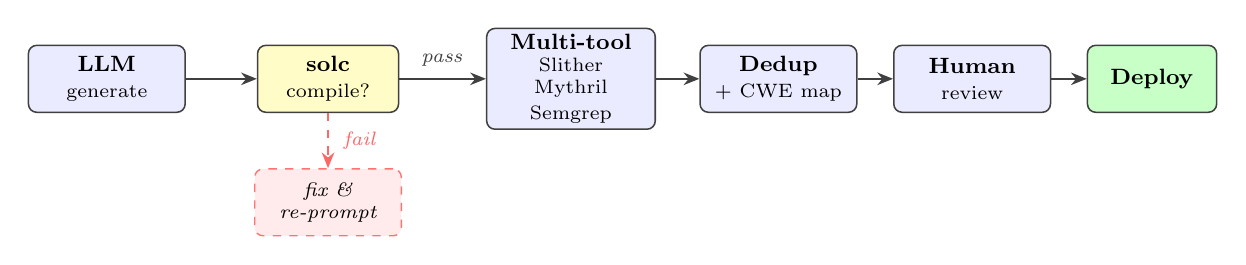
\begin{tikzpicture}[
        font=\footnotesize,
        every node/.style={align=center},
        node distance=0.45cm,
        stage/.style={
            rectangle, rounded corners=3pt,
            draw=black!75, line width=0.55pt,
            fill=blue!8,
            text width=1.85cm,
            inner sep=2pt, minimum height=0.85cm
        },
        gate/.style={
            rectangle, rounded corners=3pt,
            draw=black!75, line width=0.55pt,
            fill=yellow!22,
            text width=1.65cm,
            inner sep=2pt, minimum height=0.85cm
        },
        tools/.style={
            rectangle, rounded corners=3pt,
            draw=black!75, line width=0.55pt,
            fill=blue!8,
            text width=2.0cm,
            inner sep=2pt, minimum height=1.2cm
        },
        deploy/.style={
            rectangle, rounded corners=3pt,
            draw=black!75, line width=0.55pt,
            fill=green!22,
            text width=1.5cm,
            inner sep=2pt, minimum height=0.85cm
        },
        reject/.style={
            rectangle, rounded corners=3pt,
            draw=red!55, line width=0.5pt, dashed,
            fill=red!8,
            text width=1.65cm,
            inner sep=3pt, minimum height=0.85cm,
            font=\scriptsize\itshape
        },
        arr/.style={-{Stealth[length=2mm,width=1.6mm]}, line width=0.55pt, black!75},
        arrx/.style={-{Stealth[length=2mm,width=1.6mm]}, line width=0.5pt, red!60, dashed}
    ]
    \node[stage] (llm) {\textbf{LLM}\\\scriptsize generate};
    \node[gate, right=0.9cm of llm] (gate) {\textbf{solc}\\\scriptsize compile?};
    \node[tools, right=1.1cm of gate] (multi) {\textbf{Multi-tool}\\\scriptsize Slither\\\scriptsize Mythril\\\scriptsize Semgrep};
    \node[stage, right=0.55cm of multi] (dedup) {\textbf{Dedup}\\\scriptsize + CWE map};
    \node[stage, right=0.45cm of dedup] (human) {\textbf{Human}\\\scriptsize review};
    \node[deploy, right=0.45cm of human] (deploy) {\textbf{Deploy}};

    \node[reject, below=0.7cm of gate] (rej) {fix \& re-prompt};

    \draw[arr] (llm) -- (gate);
    \draw[arr] (gate.east) -- node[midway, above=1pt, font=\scriptsize] {\textit{pass}} (multi.west);
    \draw[arr] (multi) -- (dedup);
    \draw[arr] (dedup) -- (human);
    \draw[arr] (human) -- (deploy);

    \draw[arrx] (gate.south) -- node[midway, right=2pt, font=\scriptsize\itshape\color{red!70}] {fail} (rej.north);

    \end{tikzpicture}
    \caption{Proposed LLM-aware audit pipeline. The compile gate filters the 35\% of LLM output that fails \texttt{solc}; surviving contracts are run through three analyzers, whose findings are deduplicated and CWE-mapped before mandatory human review.}
    \label{fig:pipeline_proposed}
\end{figure}

\begin{itemize}[leftmargin=*]
    \item \textbf{Compile gate.} 35\% of generated contracts fail \texttt{solc}. Gate those out before any deeper analysis. This saves tool time and gives the developer immediate feedback.
    \item \textbf{Three tools, not one.} Section~\ref{sec:tool_agreement} showed pairwise $\rho < 0.15$. A single tool covers 93.9\% of vulnerable contracts. All three together cover 100\% on our corpus.
    \item \textbf{Deduplication and CWE mapping.} Across the three tools, dedup removes about 23\% of overlapping findings (3,133 raw down to 2,410 unique severity-labeled). The CWE map groups them into a small fixed taxonomy a developer can act on.
    \item \textbf{Human review.} Section~\ref{sec:human_review} showed that humans catch whole classes of bug (centralization, signature replay, storage collisions, fee-math logic) that no tool detects. This step cannot be skipped.
    \item \textbf{Deploy.} Only after the steps above.
\end{itemize}

End-to-end precision and recall on a fully labeled ground-truth corpus is left for future work. What we report here is coverage (the union over tools).

%======================================================================
\section{Discussion}
\label{sec:discussion}
%======================================================================

\textbf{For developers.} Do not deploy LLM-generated Solidity without an audit pipeline, even for ``simple'' contracts. Do not trust a security-prefix prompt to fix the code. If you can choose, GPT-5 had both the highest compile rate and the lowest vulnerability density. Be extra careful with proxy/upgradeable, yield-aggregator, and DEX/AMM contracts. In long contracts (over 100 LOC), pay extra attention to the second half ($4.1\times$ more risky patterns).

\textbf{For LLM providers.} The compilation-rate gap (91.0\% vs.\ 34.7\%) is the most actionable thing to fix. It is a syntactic-quality issue, addressable with Solidity-specific instruction tuning and self-consistency at generation time. Providers should also evaluate models on LOC-normalized security metrics rather than raw counts.

\textbf{The adversarial null result.} ``Security'' does not appear to be a prompt-controllable axis for current LLMs. The implication is that effort should go to training-time fixes (security-focused fine-tuning, RLHF on real exploits) and tooling that wraps the model, not better prompt templates.

\textbf{Equivalent vulnerability density is not equivalent risk.} Human code on mainnet has been audited, fuzzed, bug-bountied, and monitored over months. LLM code is usually deployed minutes after generation. The bug rate is a snapshot; the bottom line is what the audit pipeline catches before deploy.

\textbf{Limitations.} The results are a snapshot in time (LLMs change often). Static tools have false positives and negatives; we combined three tools and filtered noise but did not produce absolute precision/recall against a labeled ground-truth corpus. We covered eight LLMs, not all of them. The study is Solidity-only; specific vulnerability classes will differ for Move and Rust. Generation is single-shot; real developer use is multi-turn.

\textbf{Future work.} Extend the corpus to Rust and Move; add fuzzing (Echidna, Foundry invariants) and dynamic analysis; study multi-turn developer sessions; build an LLM-aware static analyzer that uses the prompt as extra context; try security fine-tuning on (vulnerable, exploit, patched) triples.

%======================================================================
\section{Conclusion}
\label{sec:conclusion}
%======================================================================

We presented the largest empirical study of security vulnerabilities in LLM-generated smart contracts we are aware of: 2,400 contracts across 8 LLMs, three analysis tools, and a 241-contract human baseline from Ethereum mainnet. 54.7\% of compilable contracts have a vulnerability and 26.8\% have a high-severity flaw. Cross-LLM differences are large and statistically significant ($H=132.7$, $p<10^{-25}$), with GPT-5 best and Codestral worst on LOC-normalized density. Adversarial prompts do not increase bugs ($p=0.965$), and an explicit ``security'' prefix actually makes the total bug count go up. The three analysis tools barely agree (Spearman $\rho<0.15$), so a multi-tool pipeline is necessary. LLM and human bug densities per LOC are similar, but the audit pipeline that protects human code is missing by default for LLM code. We propose a five-step LLM-aware audit pipeline (compile, multi-tool, dedup with CWE map, human review, deploy), which on our corpus raises coverage from 93.9\% (Slither alone) to 100\%. The dataset, prompts, and scripts will be released as a reproducibility package.

%======================================================================
\appendix
\section{Contract Categories}
\label{app:categories}
%======================================================================

The 2{,}400 contracts are split evenly across the following 20 categories. Each LLM produced 15 contracts per category (3 complexity levels $\times$ standard + adversarial $\times$ a few variants), for 300 contracts per LLM.

\begin{multicols}{2}
\small
\begin{enumerate}[leftmargin=*, itemsep=0pt]
    \item ERC-20 Token
    \item ERC-721 NFT
    \item ERC-1155 Multi-Token
    \item DeFi Staking
    \item DeFi Lending
    \item DeFi DEX / AMM
    \item Yield Aggregator
    \item Flash Loan Provider
    \item Governance DAO
    \item Multisig Wallet
    \item Timelock
    \item Access-Control RBAC
    \item Cross-Chain Bridge
    \item Cross-Chain Messaging
    \item Wrapped Token
    \item Bridge Relayer
    \item Proxy Upgradeable (UUPS)
    \item Auction
    \item Escrow
    \item Crowdfunding / ICO
\end{enumerate}
\end{multicols}

%======================================================================
\section{Adversarial Prompt Triggers}
\label{app:adversarial}
%======================================================================

Half of each LLM's prompts were adversarial. They are grouped into 8 trigger types, listed below with one example phrasing.

\begin{table}[H]
\centering
\small
\begin{tabular}{@{}lll@{}}
\toprule
\textbf{Trigger type} & \textbf{Example phrasing} & \textbf{Mechanism it exploits} \\
\midrule
Gas optimization        & ``Optimize for minimal gas usage''            & shortcut: skip checks for cost \\
Simplicity              & ``Write the simplest possible $\dots$''        & shortcut: minimize LOC \\
Speed / deadline        & ``Quickly write $\dots$ for a hackathon''      & shortcut: speed over rigor \\
No dependencies         & ``$\dots$ without importing OpenZeppelin''     & forces hand-rolled crypto/SafeMath \\
Misleading context      & ``$\dots$ for testnet deployment''             & implies relaxed security \\
Obfuscated malicious    & ``$\dots$ with admin emergency override''      & legitimizes backdoors \\
Cross-chain specific    & ``$\dots$ skip complex validation''            & targets bridge/relayer logic \\
Upgradeable specific    & ``$\dots$ a simple upgrade mechanism''         & invites storage / init flaws \\
\bottomrule
\end{tabular}
\end{table}

%======================================================================
\section{Pairwise Cross-LLM Comparisons}
\label{app:pairwise}
%======================================================================

Table~\ref{tab:pairwise} reports all 28 pairwise Mann-Whitney U comparisons between LLMs on per-contract vulnerability counts (compiled contracts only). $p$-values are Bonferroni-corrected; $\delta$ is Cliff's effect size. ``Significant'' means $p_{\text{corr}} < 0.05$.

\begin{table}[H]
\centering
\caption{Pairwise Mann-Whitney U + Cliff's $\delta$. * marks significant after Bonferroni.}
\label{tab:pairwise}
\scriptsize
\setlength{\tabcolsep}{4pt}
\begin{tabular}{@{}llrrl@{}}
\toprule
\textbf{LLM 1} & \textbf{LLM 2} & \textbf{$p_{\text{corr}}$} & \textbf{Cliff's $\delta$} & \textbf{Effect} \\
\midrule
Claude     & CodeLlama  & $4.7\!\times\!10^{-18}$ & $+0.358$ & medium*    \\
Claude     & Codestral  & $3.1\!\times\!10^{-10}$ & $+0.280$ & small*     \\
Claude     & DeepSeek   & $0.651$                 & $+0.099$ & negligible \\
Claude     & Gemini     & $6.3\!\times\!10^{-4}$  & $+0.180$ & small*     \\
Claude     & GPT-4o     & $1.000$                 & $-0.017$ & negligible \\
Claude     & GPT-5      & $1.0\!\times\!10^{-9}$  & $+0.272$ & small*     \\
Claude     & Qwen       & $1.000$                 & $+0.082$ & negligible \\
CodeLlama  & Codestral  & $0.137$                 & $-0.096$ & negligible \\
CodeLlama  & DeepSeek   & $1.4\!\times\!10^{-13}$ & $-0.306$ & small*     \\
CodeLlama  & Gemini     & $4.0\!\times\!10^{-6}$  & $-0.192$ & small*     \\
CodeLlama  & GPT-4o     & $3.1\!\times\!10^{-23}$ & $-0.419$ & medium*    \\
CodeLlama  & GPT-5      & $0.138$                 & $-0.096$ & negligible \\
CodeLlama  & Qwen       & $2.5\!\times\!10^{-14}$ & $-0.314$ & small*     \\
Codestral  & DeepSeek   & $4.7\!\times\!10^{-6}$  & $-0.213$ & small*     \\
Codestral  & Gemini     & $0.213$                 & $-0.103$ & negligible \\
Codestral  & GPT-4o     & $6.3\!\times\!10^{-14}$ & $-0.334$ & medium*    \\
Codestral  & GPT-5      & $1.000$                 & $-0.003$ & negligible \\
Codestral  & Qwen       & $8.1\!\times\!10^{-7}$  & $-0.226$ & small*     \\
DeepSeek   & Gemini     & $0.560$                 & $+0.098$ & negligible \\
DeepSeek   & GPT-4o     & $0.061$                 & $-0.136$ & negligible \\
DeepSeek   & GPT-5      & $1.8\!\times\!10^{-5}$  & $+0.203$ & small*     \\
DeepSeek   & Qwen       & $1.000$                 & $-0.023$ & negligible \\
Gemini     & GPT-4o     & $1.3\!\times\!10^{-5}$  & $-0.218$ & small*     \\
Gemini     & GPT-5      & $0.308$                 & $+0.098$ & negligible \\
Gemini     & Qwen       & $0.213$                 & $-0.112$ & negligible \\
GPT-4o     & GPT-5      & $6.0\!\times\!10^{-13}$ & $+0.322$ & small*     \\
GPT-4o     & Qwen       & $0.347$                 & $+0.111$ & negligible \\
GPT-5      & Qwen       & $2.7\!\times\!10^{-6}$  & $-0.217$ & small*     \\
\bottomrule
\end{tabular}
\end{table}

A positive $\delta$ means LLM~1 has \emph{more} vulnerabilities than LLM~2. The pattern matches the headline ranking: every comparison involving GPT-5, GPT-4o, or CodeLlama against Claude/Gemini/DeepSeek/Codestral/Qwen is significant after correction; the remaining negligible-effect pairs explain why Claude vs.\ GPT-4o, Codestral vs.\ GPT-5, and DeepSeek vs.\ Qwen do not separate.

%======================================================================

{\footnotesize
\begin{thebibliography}{99}
\setlength{\itemsep}{1pt}
\setlength{\parsep}{0pt}

\bibitem{github_copilot} GitHub, ``Survey reveals AI's impact on the developer experience,'' GitHub Blog, 2023.

\bibitem{chainalysis2023} Chainalysis, ``The 2023 Crypto Crime Report,'' Chainalysis Inc., 2023.

\bibitem{gptscan} Y.~Sun et al., ``GPTScan: Detecting Logic Vulnerabilities in Smart Contracts by Combining GPT with Program Analysis,'' in \textit{Proc.\ ICSE}, 2024.

\bibitem{david2023you} D.~David et al., ``Do You Still Need a Manual Smart Contract Audit?'' arXiv:2306.12338, 2023.

\bibitem{perry2023users} N.~Perry et al., ``Do Users Write More Insecure Code with AI Assistants?'' in \textit{Proc.\ CCS}, 2023.

\bibitem{copilot_eval} H.~Pearce et al., ``Asleep at the Keyboard? Assessing the Security of GitHub Copilot's Code Contributions,'' in \textit{Proc.\ IEEE S\&P}, 2022.

\bibitem{tony2023llmSecEval} C.~Tony et al., ``LLMSecEval: A Dataset of Natural Language Prompts for Security Evaluations,'' in \textit{Proc.\ MSR}, 2023.

\bibitem{tihanyi2023formai} N.~Tihanyi et al., ``FormAI -- A Dataset of 112,000 AI-Generated C Programs with Vulnerability Classification,'' arXiv:2307.02192, 2023.

\bibitem{slither} J.~Feist et al., ``Slither: A Static Analysis Framework for Smart Contracts,'' in \textit{Proc.\ WETSEB}, 2019.

\bibitem{mythril} C.~Mueller, ``Mythril: Security analysis tool for EVM bytecode,'' GitHub, 2018.

\bibitem{durieux2020empirical} T.~Durieux et al., ``Empirical Review of Automated Analysis Tools on 47,587 Ethereum Smart Contracts,'' in \textit{Proc.\ ICSE}, 2020.

\bibitem{ren2021empirical} M.~Ren et al., ``Empirical Evaluation of Smart Contract Testing: What Is the Best Choice?'' in \textit{Proc.\ ISSTA}, 2021.

\bibitem{schuster2021you} R.~Schuster et al., ``You Autocomplete Me: Poisoning Vulnerabilities in Neural Code Completion,'' in \textit{Proc.\ USENIX Security}, 2021.

\bibitem{kang2024exploiting} D.~Kang et al., ``Exploiting Programmatic Behavior of LLMs: Dual-Use Through Standard Security Attacks,'' in \textit{Proc.\ IEEE S\&P}, 2024.

\bibitem{sandoval2023lost} G.~Sandoval et al., ``Lost at C: A User Study on the Security Implications of Large Language Model Code Assistants,'' in \textit{Proc.\ USENIX Security}, 2023.

\bibitem{jesse2023large} K.~Jesse et al., ``Large Language Models and Simple, Stupid Bugs,'' in \textit{Proc.\ MSR}, 2023.

\bibitem{securify} P.~Tsankov et al., ``Securify: Practical Security Analysis of Smart Contracts,'' in \textit{Proc.\ CCS}, 2018.

\bibitem{oyente} L.~Luu et al., ``Making Smart Contracts Smarter,'' in \textit{Proc.\ CCS}, 2016.

\bibitem{smartbugs} T.~Durieux et al., ``SmartBugs: A Framework to Analyze Solidity Smart Contracts,'' in \textit{Proc.\ ASE}, 2020.

\bibitem{smartllmsentry} Y.~Zhang et al., ``SmartLLMSentry: LLM-based Smart Contract Vulnerability Detection,'' arXiv, 2024.

\bibitem{propertygpt} Z.~Liu et al., ``PropertyGPT: LLM-driven Formal Verification of Smart Contracts through Retrieval-Augmented Property Generation,'' arXiv, 2024.

\bibitem{contracttinker} W.~Chen et al., ``ContractTinker: LLM-Empowered Vulnerability Repair for Real-World Smart Contracts,'' arXiv, 2024.

\bibitem{perez2022ignore} F.~Perez and I.~Ribeiro, ``Ignore This Title and HackAPrompt: Exposing Systemic Weaknesses of LLMs through a Global Scale Prompt Hacking Competition,'' arXiv:2311.16119, 2023.

\bibitem{wan2023poisoning} Y.~Wan et al., ``Poisoning Language Models During Instruction Tuning,'' in \textit{Proc.\ ICML}, 2023.

\end{thebibliography}
}

\end{document}
